\documentclass{article}
\usepackage{graphicx}
\usepackage[english]{babel}
%\usepackage[a4paper]{geometry}
\usepackage[utf8]{inputenc}
\usepackage[T1]{fontenc}
\usepackage{needspace}
\usepackage{marginnote}
\renewcommand*{\marginfont}{\sffamily\footnotesize}
\usepackage{hyperref, graphicx, wrapfig}
\usepackage{imakeidx}
\usepackage{hyperref}
\makeindex[intoc]
\usepackage{pdfpages}
\usepackage{multirow}
\usepackage{color}
\usepackage{xcolor,colortbl}

\usepackage{tikz}
\usetikzlibrary{positioning}

\definecolor{Red}{rgb}{1,0,0}
\definecolor{Green}{rgb}{0,1,0}
\usepackage{tabularx}
\usepackage{caption}
\usepackage{background}

\backgroundsetup{
scale=1,
angle=34,
opacity=0.4,
contents={
\begin{tikzpicture}[remember picture,overlay]
 \path [left color = red!45,middle color = red!35, right color = white,rotate=1] (current page.south west)rectangle (current page.north east);   % Adjust the position of the logo.
\end{tikzpicture}\begin{tikzpicture}[remember picture,overlay]
 \path [left color = white,middle color = blue!20, right color = blue!40,rotate=13] (current page.south west)rectangle (current page.north east);   % Adjust the position of the logo.
\end{tikzpicture}\begin{tikzpicture}[remember picture,overlay]
 \path [left color = white,middle color = yellow!30, right color = white ,rotate=-13] (current page.south west)rectangle (current page.north east);   % Adjust the position of the logo.
\end{tikzpicture}}
}
%\newenvironment{overview}[3][]{
%  \needspace{10\baselineskip}
%  \begin{center}
%    { \renewcommand\textsuperscript[1]{}
%      \phantomsection\addcontentsline{toc}{section}
%      {\texorpdfstring{#2 (\emph{#3})}{#2 (#3)}}
%    }
%    {\large\bfseries #2\\}
%    \medskip
%    {#3\par}
%    \smallskip
%
%
%  {%
%  \bigskip
%  \hrule
%  \bigskip
%  }
%
%  \end{center}
%}
\newenvironment{overview}[4][]{
  \needspace{10\baselineskip}
  \begin{center}
    { \renewcommand\textsuperscript[1]{}
      \phantomsection\addcontentsline{toc}{section}
      {\texorpdfstring{#2 (\emph{#3})}{#2 (#3)}}
    }
    {\large\bfseries #2\\}
    \medskip
    {#3\par}
    \smallskip
    {\small #4\par}

  {%
  \bigskip
  \hrule
  \bigskip
  }
  \end{center}
}

\newcommand{\mc}[2]{\multicolumn{#1}{c}{#2}}
\newcommand{\mlcr}[4]{\multicolumn{#1}{#4}{\multirow{#2}{*}{#3}}}

\tikzstyle{blue} = [rectangle, draw, fill=blue!20,
 text width=0.4\textwidth, text centered, minimum height=4em]

\tikzstyle{red} = [rectangle, draw, fill=red!20,
 text width=0.4\textwidth, text centered, minimum height=4em]

\tikzstyle{timered} = [rectangle, draw, fill=red!20,
 text width=0.1\textwidth, text centered, minimum height=4em]

\tikzstyle{timeblue} = [rectangle, draw, fill=blue!20,
 text width=0.1\textwidth, text centered, minimum height=4em]

\tikzstyle{blue2} = [rectangle, draw, fill=blue!20,
 text width=0.4\textwidth, text centered, minimum height=6em]

\tikzstyle{red2} = [rectangle, draw, fill=red!20,
 text width=0.4\textwidth, text centered, minimum height=6em]

\tikzstyle{timered2} = [rectangle, draw, fill=red!20,
 text width=0.1\textwidth, text centered, minimum height=6em]

\tikzstyle{timeblue2} = [rectangle, draw, fill=blue!20,
 text width=0.1\textwidth, text centered, minimum height=6em]


\begin{document}

\newenvironment{changemargin}[2]{%
\begin{list}{}{%
\setlength{\topsep}{0pt}%
\setlength{\leftmargin}{#1}%
\setlength{\rightmargin}{#2}%
\setlength{\listparindent}{\parindent}%
\setlength{\itemindent}{\parindent}%
\setlength{\parsep}{\parskip}%
}%
\item[]}{\end{list}}

\begin{titlepage}
	\centering
	
\includegraphics[width=0.8\textwidth]{img/mat-mn-navn-eng.eps}\par\vspace{1cm}
	{\scshape\LARGE Bio-mechanics workshop on cell membrane dynamics, active matter and plasticity in tissue \par}
	\vspace{1cm}
	{\scshape\Large Tøyen Hovedgård \\ Oslo Norway\par}
	\vspace{1.5cm}

\begin{changemargin}{-1cm}{-1cm}

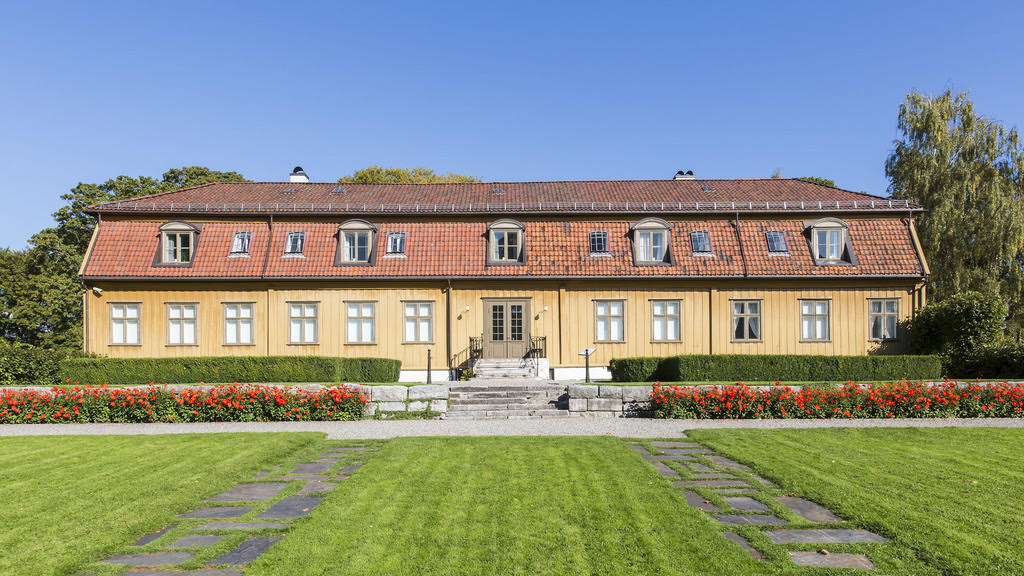
\includegraphics[scale=0.4]{img/hoved.jpg}

\centering
\vspace{0.5cm}
%{\scshape\Large  Sponsors}
\vspace{0.5cm}




\includegraphics[scale=0.45]{img/UiO_Seal_B_ENG_cmyk.eps}\hspace*{2cm}
%
\includegraphics[scale=0.45]{img/logo.png}
\end{changemargin}

	\vfill

% Bottom of the page

\end{titlepage}


















\newcommand{\eventblock}[5]{
\node [#1,#2] (#3) {#4};
\node [time#1,left= of #3] (Time) {#5 }  ;  }
\begin{center}
\section*{PROGRAM}
\begin{changemargin}{-1cm}{-1cm}

\begin{tikzpicture}[node distance=-1pt, auto]
 % Place nodes

\eventblock{red}{}{Friday}{Program \\ Friday August 30 }{}
\eventblock{blue}{below= of Friday}{Registration}{Registration with coffee and pastry}{09.30\\(09:30)}
\eventblock{red}{below= of Registration}{Opening}{Opening}{09.45\\(09:45)}
\eventblock{blue}{below= of Opening}{SessionOne}{Paul Dommersnes\\
Amin Doostmohammadi}{S1 \\ 10.00\\(10:00)}
\eventblock{red}{below= of SessionOne}{BreakOne}{Break with coffee and softdrinks}{10.50\\(11:00)}
\eventblock{blue2}{below= of BreakOne}{SessionTwo}{Paolo Zunino\\ Alessandro Colcite\\Federico Fenarilo(?)}{S2 \\ 11.10\\(11:20)}
\eventblock{red}{below= of SessionTwo}{Lunch}{Lunch}{12.25\\(12:50)}
\eventblock{blue}{below= of Lunch}{SessionThree}{Jaques Prost\\Susanne Liese}{S3 \\ 13.30\\(13:50)}
\eventblock{red}{below= of SessionThree}{BreakTwo}{Break with coffee and fruits}{14.20\\(15:20)}
\eventblock{blue2}{below= of BreakTwo}{SessionFour}{Kartik Jain\\Hunter King\\Corinna Maass}{S4 \\ 14.40\\(15:40)}
\eventblock{red}{below= of SessionFour}{Social}{Social gathering with snacks, beer and wine.}{15.55\\(17:00)}
\eventblock{blue}{below= of Social}{Dinner}{Workshop dinner at \\ Solsiden}{19.00\\(19:00)}


\eventblock{red}{right=2cm of Friday}{Saturday}{Program \\ Saturday August 31 }{}
\eventblock{blue2}{below= of Saturday}{SessionFive}{Jakob Schreiner\\ Vegard Vinje\\Alain Goriley }{S5 \\ 09.30\\(09:30)}
\eventblock{red}{below= of SessionFive}{BreakThree}{Break with coffee, croissants and softdrinks}{  10.45\\(11:00)}
\eventblock{blue2}{below= of BreakThree}{SessionSix}{Kaare Hartvig-Jensen\\NN (Cinzia Progida)\\ Emma L\aa ng }{S6 \\ 11.05\\(11:20)}
\eventblock{red}{below= of SessionSix}{LunchTwo}{Lunch}{12.20\\(12:50)}
\eventblock{blue}{below= of LunchTwo}{Tour}{Guided Tour Botanical Garden }{13.30\\(13:50)}


\end{tikzpicture}
\end{changemargin}
\end{center}

\clearpage

\
\subsection*{\underline{The airport}}

\textbf{When you arrive at the airport} you need to
get to Oslo city center (Oslo S).
The fastest and easiest means of transportation to and from the airport
is by train. There are two different train operators, NSB
(Norwegian State Railway) and Flytoget (Airport Express Train).
There are some differences in price and
 and frequency of departures.
\textbf{Tickets for both NSB and Flytoget} can be bought at the airport
and at Oslo S in automatic ticket machines which accepts both cash
and credit cards.

\textbf{Traveling with NSB} is the cheapest
option whit a single ticket price
of 93 NOK. The frequency of departures varies but
usually there are at least 2 per hour and the time of travel is 23
 minutes. The times for departure is easy to find
both at the airport and at Oslo S.
At NSB it is also possible to buy your ticket
onboard the train at an additional cost of $40$NOK.
Pay attention to which stop to exit at (Oslo S/Gardermoen airport)
as this might not be the end stop for the train.

\textbf{Traveling with Flytoget} costs 180 NOK for a single ticket
but the frequency of departure per hour is 6, one every
ten minutes with a travel time of approximately 20 minutes.
Flytoget does not accept on-board payment!


\subsection*{\underline{Getting around in Oslo}}

The public transportation in Oslo is good with frequent
departures if you want
to take a bus, tram or subway. Buying tickets must be
done in advance and there are many places you can buy a
ticket. Oslo S, Narvesen, 7-eleven and Deli de Luca are some of the places.
A short "how-to" guide for getting to and from your hotel
 to the workshop related
locations (Fig.\ref{fig:Oslo}) follows below. Keep in mind that
the distances
between the different locations are not very large so if the
weather is nice, walking is recommended. If needed, taxi's
are a common sight in Oslo but if none are found you can order one
at tlf: +47 02323. Note that taxies are expensive in Norway.

%\clearpage

\subsection*{\underline{Comfort Hotel Karl Johan}}

\begin{wrapfigure}{r}{0.4\textwidth}
\centering
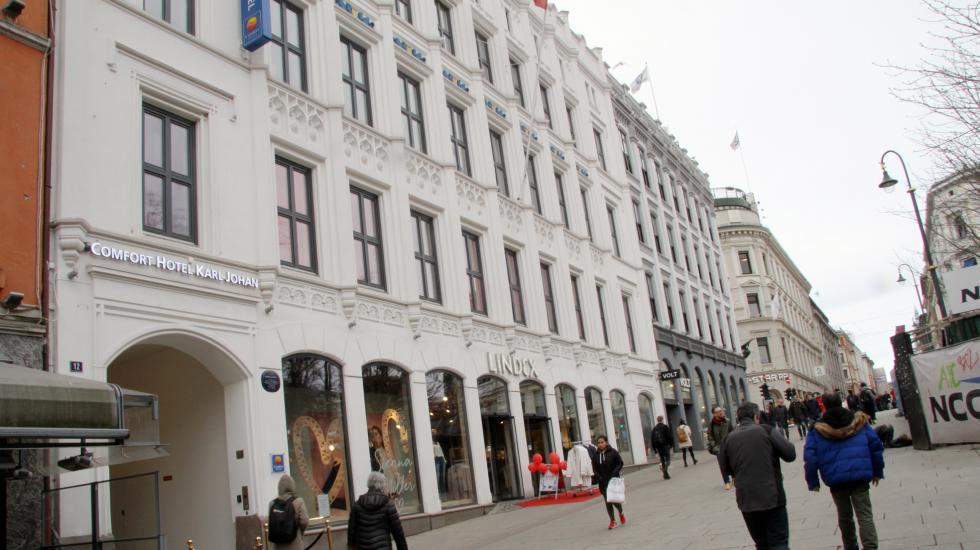
\includegraphics[scale=0.2]{img/comfort_karl_johan.jpg}
\caption{\label{fig:frog1}Exterior of Comfort Hotel Karl Johan.}
\end{wrapfigure}
The hotel is located at Karl Johans gate 12 near
the train station at Jernbanetorget.
This is also
a hub for public transportation in Oslo. \textbf{To get to
Tøyen hovedgård} where the workshop is taking place,
the best option is to take the subway from Jernbanetorget
to Tøyen and walk the remaining bit. The subway station
at Jernbanetorget is located under the shopping centre
Byporten and the entrances are clearly marked.
All subway trains,
\noindent 1-5, go to Tøyen from
Jernbanetorget in the eastward direction. \textbf{To get from
the restaurant, Trattoria Popolare,} you can take the tram. Lines
11, 12 and 13 will take you from Schous Plass to Jernbanetorget.


\clearpage
\begin{center}


%WHAT TO DO
\section*{What to do in Oslo ?}
In Oslo there are many different tourist attractions, and we will present a few  popular sites. Attractions in Oslo can be found on \href{www.visitoslo.com}{www.visitoslo.com}.


\end{center}
\begin{wrapfigure}[9]{R}{0.5\textwidth}
    \centering
    \captionsetup{width=0.4\textwidth}
    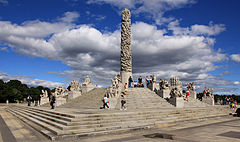
\includegraphics[width=0.5\textwidth]{img/Vigelansparken.jpg}%
     \caption{The monolith sculpute in the Park.}
\end{wrapfigure}

\section*{Vigeland Sculpture Park}

Vigeland Park is the world's largest sculpture park made by a single artist, and is one of Norway's most popular tourist attractions. The unique sculpture park is Gustav Vigeland's lifework with more than 200 sculptures in bronze, granite and wrought iron. The park is located a short 10 minute walk from the subway station Majorstuen.

\begin{wrapfigure}[10]{R}{0.5\textwidth}
    \centering
    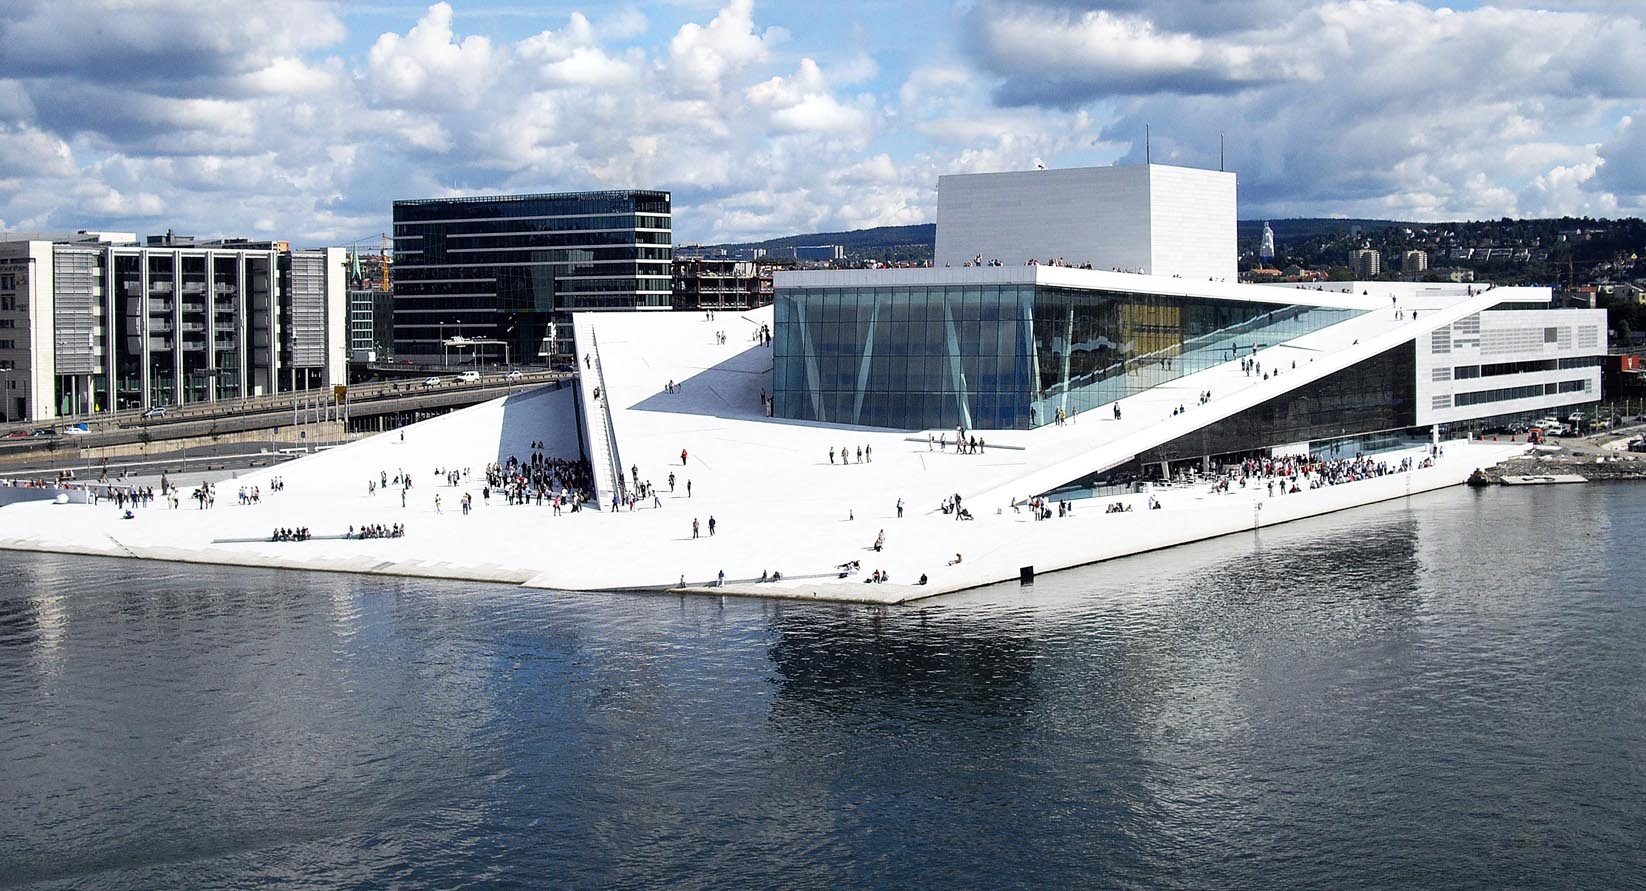
\includegraphics[width=0.5\textwidth]{img/operahouse.jpg}%
     \caption{Oslo Opera House }
\end{wrapfigure}

\vspace{1cm}

\section*{Opera House}
Oslo's Opera House is located right at the harbour, with an angled, white exterior that appears to rise from the water. It invites its visitors to climb its roof and enjoy panoramic views of Oslo and the fjord, all year round. \\
Large-scale windows at street level provide the public with glimpses of rehearsals and workshop activities. The building's interior is mainly oak, and the main hall is shaped like a horseshoe, reminiscent of classical theatres of the past. The opera is designed by the Norwegian architecture firm Snøhetta, and has received several prestigious awards. You can walk to the Opera House from the Jernbanetorget (central station) in about 15 minutes.

\clearpage

\section*{Gr\"unerløkka}
Through Oslo, from north to south, runs the river Akerselva. Along the river there are parklands and walking trails, but also remains of Oslo’s industrial history.
Gr\"unerløkka lies on the east side of the river, behind the old industrial buildings. The former factory district turned fashion hub, with laid-back cafes and galleries galore, Gr\"unerløkka is a colourful mix of old and new decor. Independent boutiques and design shops showcase Oslo’s more alternative side, with 19th-century buildings serving as a picturesque backdrop.

\bigskip
\bigskip

\begin{figure}[h]
    \centering
    \href{https://www.google.com/maps/d/edit?hl=no&hl=no&mid=1q9FpcHekR77D16V4eefgqkybvNc&ll=59.91839077669053%2C10.758429782339476&z=15}{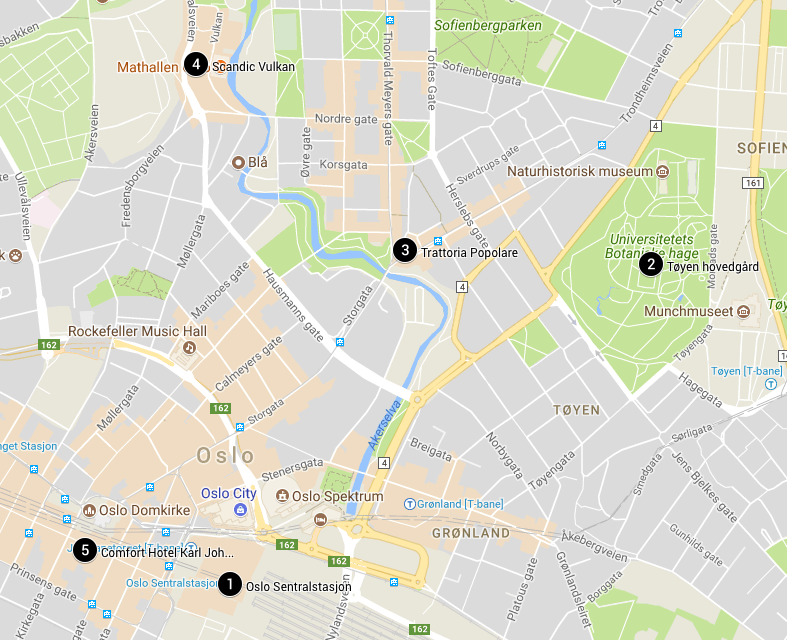
\includegraphics[width=1\linewidth, height=1\linewidth]{img/Oslo.png}}
    \caption{Locations of the 5 workshop related locations in Oslo.}
    \label{fig:Oslo}
\end{figure}




\clearpage



% ABSTRACTS

\includegraphics[scale=0.3]{img/mat-mn-navn-eng.eps}


\section*{Session 1}
\overview{State transitions in synthetic active matter}
{Paul Dommersnes\textsuperscript{1} \& Jon Otto Fossum\textsuperscript{1,2}}
{\textsuperscript{1}Department of Physics, Norwegian University of Science and Technology (NTNU) Høgskoleringen 5, N-7491 Trondheim, Norway \newline
    \textsuperscript{2}Institut Pierre-Gilles de Gennes (IPGG), 6-12 rue Jean Calvin, Paris 75005, France}
{Biological active matter, such as populations of cells and animals, often change between
different swarming states. One example is shoaling, milling and schooling fish. Synthetic
active matter consist of self-propelled inanimate units and emulates biological active matter.
We combine electric field induced attraction with electro-rolling propulsion [1] in a
population of granular beads. A variety of swarming regimes is realized: living clusters, a stripe
phase of clusters, and polar liquid swarms, reminiscent of transitions seen in active matter
simulations [2,3,4]. Remarkably, the crystal to liquid transition occurs at a different velocity
threshold than the local to global polar order transition. The experimental system offers a
physical model for swarming transitions in biological active matter, and can also open new
routes for controlling self-assembly in soft matter technologies.\newline\newline
\small{
[1] A. Bricard, J.-B. Caussin, N. Desreumaux, O. Dauchot, D. Bartolo, Emergence of macroscopic
directed motion in populations of motile colloids, Nature 503, 95 (2013)\newline
[2] Living Clusters and Crystals from Low-Density Suspensions of Active Colloids, B. M. Mognetti, A.
Šarić, S. Angioletti-Uberti, A. Cacciuto, C. Valeriani, and D. Frenkel, Phys. Rev. Lett. 111, 245702 – (2013)\newline
[3] Hydrodynamic interactions in dense active suspensions: From polar order to dynamical clusters,
N. Yoshinaga and T. B. Liverpool Phys. Rev. E 96, 020603(R) (2017)\newline
[4] Spontaneous aggregation and global polar ordering in squirmer suspensions
F.Alarcón and I.Pagonabarraga, Journal of Molecular Liquids, 185, Pages 56-61 (2013)}}

\overview{Active Thin structures}
{Amin Doostmohammadi}
{The Rudolf Peierls Centre for Theoretical Physics, University of Oxford, UK}
{Monolayers of cells in tissue are examples of thin structures that are continuously driven out of
equilibrium by the activity of their constituent elements. One generic property of these active
layers is the spontaneous emergence of collective flows which often leads to chaotic flow patterns
characterised by swirls, jets, and topological defects in their orientation field [1]. In this talk I
will discuss recent works on cell monolayers, where we find interesting correlations between liquid
crystal-like features of these active systems and their biological functionality.
I will explain our recent finding on the role of topological defects in regulating the morphology of
growing cell colonies and represent evidence on spontaneous formation of singularities in cellular
alignment in the form of nematic topological defects, as a previously unidentified cause of cell
apoptosis and extrusion, suggesting that such defects govern cell fate in epithelial tissues [2,3]. In
addition, I will present the emergence of tissue-scale oscillations in epithelial tissues when confined
within micro-domains [4].\newline\newline
\small{
[1] A. Doostmohammadi, J. Ignés-Mullol, J. M. Yeomans, F. Sagués, Active nematics. Nature
Communications, 9:3246, 2018.\newline
[2] T. B. Saw, A. Doostmohammadi, et al., Topological defects in epithelia govern cell death and
extrusion. Nature, 544.7649: 212-216, 2017.\newline
[3] R. Mueller, J. M. Yeomans, A. Doostmohammadi, Emergence of active nematic behavior in
monolayers of isotropic cells. Physical Review Letters, 122:048004, 2019.\newline
[4] G. Peyret, R. Mueller, J. DeAlessandro, S. Begnaud, P. Marcq, R. Mége, J. M. Yeomans,
A. Doostmohammadi, B. Ladoux, Sustained oscillations in epithelial cell sheets. Biophysical
Journal, 6:464–478, 2019.}}

\newpage
\section*{Session 2}

% \overview{}{Paolo Zunino}{}{}

\overview{A Lattice-Boltzmann-Immersed Boundary technique for computing the vascular journey of micro-particles}
{Allesandro Coclite}
{School of Engineering Università degli Studi della Basilicata}
{Micro and nano–particles are systemically injected as drug carriers to specifically
deliver therapeutics into diseased tissue. Their vascular journey and adhesion mechanics
are key ingredient to optimize strategies mainly against cancer and cardiovascular
disorders. Computational methods are crucial to deep understand the vascular transport of
platelets-like objects due to the large number of parameters involved. Particles can be
precisely tailored in term of their shape, size, superficial properties and stiffness
(the so called 4S parameters) to modulate their abilities, so that, the number of paths
toward the optimization uncontrollably grows. The recipe for efficient micro- and
nano-carriers, in particular, is far from being discovered and computational model are
useful tools for the design of such constructs. Indeed, reliable computational schemes
must account for the transport of several structures with different stiffness, densities,
shapes, and need to model particle-particle and particle-walls interactions.  Here, a
kinematic/dynamics hybrid Immersed–Boundary (IB)/Lattice Boltzmann (LB) scheme is
proposed. Coclite et al. (2019) Precisely, the IB technique is employed in its kinematic
formulation for the red blood cells in order to save computational time. Red cell
membranes are considered here as dense as plasma, so that, the membranes velocity is
advected with the withstanding fluid velocity. On the contrary, microparticles are
transported with the dynamics IB formulation developed and validated by the author.
Coclite et al. (2018, 2019) Both, cells and microcarriers are modeled as a collection of
mass-spring elements responding to a bending potential, a worm-like chain potential and
the area conservation constraint. Furthermore, on particles’ surfaces are uniformly
distributed adhesive molecules (ligands) interacting with their counterpart (receptors)
disposed on vascular walls.\newline\newline
\small{A. Coclite, S. Ranaldo, M.D. de Tullio, P. Decuzzi, and G. Pascazio. Kinematic
and dynamic forcing strategies for predicting the transport of inertial capsules via a
combined lattice boltzmann immersed boundary method. Computers \& Fluids, 180:
41–53, 2019. ISSN 0045-7930. doi: https://doi.org/10.1016/j.compfluid.2018.12.014.\newline
A. Coclite, G. Pascazio, M.D. de Tullio, and P. Decuzzi. Predicting the vascu-
lar adhesion of deformable drug carriers in narrow capillaries traversed by blood
cells. Journal of Fluids and Structures, 82:638 – 650, 2018. ISSN 0889-9746. doi:
https://doi.org/10.1016/j.jfluidstructs.2018.08.001.}}

\overview{Using the zebrafish for analyzing the flow of nanoparticles into the blood.}
{Federico Fenaroli}
{University of Oslo, Section for Physiology and Cell Biology}
{Delivering drugs via nano-sized carriers is set to change the way we treat diseases in the coming decades.
The zebrafish embryo, unlike the mouse, is a model ideally suited for visualizing nanoparticles at high
resolution in a live animal. Its optical transparency and genetic versatility allow real time observations of
vascular flow of nanoparticles and their interactions with cells throughout the body. Consequently, this
system enables the acquisition of quantitative data that are difficult to obtain in rodents. In particular, we
have developed automated quantitative methods for analyzing important parameters of nanoparticle behavior,
such as circulation time and interactions with key target cells, macrophages and endothelial cells. Our
results show that nanoparticles having long or short blood circulation in rodents behave similarly in the
zebrafish embryo, in a manner that is strongly influenced by uptake into macrophages or endothelial cells.
Moreover fast recording of nanoparticles flowing in the blood of zebrafish allowed, via PTV
(particle tracking velocimetry), an analysis of how nanocarriers circulate with respect to the endothelium; an
important parameter considered to be crucial for predicting the accumulation of nanoparticles at diseased sites.  }

\newpage
\section*{Session 3}

\overview{Emergence and resurgence in elementary contractile unit}
{Jaques Prost \& J F Rupprecht}
{Mechanobiology Institute, National University of Singapore, 5A Engineering Drive 1, 117411 (Singapore).
Laboratoire Physico Chimie Curie, Institut Curie,
PSL Research University, CNRS UMR168, 75005 Paris, France}
{After introducing the main features characterizing an elementary contractile unit in cells,
I will recall theoretical results concerning motor collections obtained over the years.
In particular I will show how a symmetry breaking transition, emergent feature of a large
number of molecular motor collection, underpins a wide number of biological functions from
muscle oscillations to sound detection.  I will then show how a simple modification of the
theoretical framework allows to understand all experimental observations including force
build-up followed by a relaxation and the existence of half integer steps in the
contraction/relaxation curve, which is a resurgence of a nanoscopic scale in a mesoscopic
system.}

\overview{Protein Crowding mediates Passive Membrane Remodeling in ESCRT induced Intraluminal Vesicles Formation }
{Susanne Liese}
{Department of Mathematics, University of Oslo}
{Transmembrane proteins are sorted by the endosomal sorting complex required for transport (ESCRT) machinery
into intraluminal vesicles (ILVs). Vesicle formation starts with a small deformation of the endosome membrane,
which grows in time and leads to the formation of an ILV. We present a minimal mathematical model that
describes ILV formation as a result of the interplay between protein induced Gaussian bending rigidity and
protein crowding. The model reproduces several key experimental findings: (1) An ESCRT-free ILV is formed with
(2) a diameter that is independent of the endosome size and (3) an enhanced ESCRT density in the membrane neck
region. We find that all three observations, are a consequence of an energy minimization, which balances the
loss in binding energy in the ESCRT-free ILV bud by a gain in Gaussian bending energy in the membrane neck
region. Furthermore, we find that a passive ILV formation, which follows a negative energy gradient, is
enabled by a non-homogenous Gaussian bending rigidity, due to the crowding of ESCRT proteins in the membrane
neck. Combining the mathematical model with experimental measurements of ESCRT recruitment dynamics and 
electron microscopy imaging of transient ILV shapes, we discuss the role of so-called early ESCRTs in membrane
shape remodeling, which supports the notion that early ESCRTs cause membrane budding by protein crowing
without ATP consumption.}

\newpage
\section*{Session 4}

\overview{Computational Modeling of Bacterial Dynamics}
{Kartik Jain}
{Institute for Computational Physics, University of Stuttgart, Allmandring 3, 70569 Stuttgart}
{Microorganisms namely bacteria can propel, proliferate and form aggregations in a number
of media, and they exhibit interesting behavior under shear flow field. In addition to being self-
propelled, some bacteria can adhere to each other and to surfaces where they can create fast
growing colonies, called biofilms. Extensive research efforts focus on understanding of the life cycle
of a biofilm i.e. ranging from collective bacterial dynamics to biofilm formation and its depletion.
Biofilm research has applications in various fields like biology, medicine and engineering. Studies
have demonstrated that bacteria more commonly accumulate at surfaces and around obstacles that
they encounter in their propulsion path. The initiation, growth and decline of a biofilm depends
largely on the flow field and forces that are acting on them.
Computational modeling has evolved as an important tool for the study of physical and biological
phenomena whereby mathematical models of a process are developed and studied using simulations
on computers. In this work, we developed a model to study the dynamics of Escherichia Coli
(E. Coli) bacteria to study their growth, replication, adherence to surfaces under shear flow. In
the model the bacteria are represented by molecular dynamics (MD) particles while the fluid is
represented by a lattice Boltzmann method (LBM). The MD particles are coupled to the LB
fluid using a frictional point coupling that ensures momentum conservation of the total system.
We present collective transient dynamics of up to 4000 bacteria in confined geometries with and
without external flow. All the simulations are performed on one GPU using the ESPResSo package
for soft matter, each requiring about 108 hours of execution time. Our results show ephemeral
accumulation of bacteria around obstacles, and their tendency to undergo a momentary stasis in
the regions of flow recirculations. We further model bacterial replication whereby one bacterium
replicates to about 2 16 dynamically in the simulation to form a large colony, which, under the
effect of shear forces washes away eventually. The model is currently being parametrized using
experimental data and ongoing research will include application of this model to study microbial
growth under gradients of nutrition.}

\overview{Insect strategies for atmospheric water harvesting}
{Hunter King}
{Department of Polymer Science, University of Akron}
{Where water is scarce, living systems will exploit sometimes unexpected physical
mechanisms to meet their inflexible demand for it. In regions lacking consistent
precipitation, their strategies to capture water from the atmosphere can be particularly
suited for translation for sustainable engineering. I will present two sources of
inspiration to this end: Beetles of the Namib desert famously lean into foggy wind to
collect water. The dominant narrative regarding their adaptation in recent literature is
one of tuned wettability for surface transport, without reference to primary, fluid
mechanisms by which droplets reach the surface in the first place.  We explore, with
table-top experiment and synthetic analogs, an alternative story, by which surface
morphology enhances deposition efficiency. Mounds of the fungus cultivating termite
species use architecture to alternatively dampen and harness external thermal oscillations
for thermoregulation and convective internal ventilation, respectively. However, their
demands for both respiration and high humidity put their physiology at odds with the arid
environments where they are prolific, and a clear understanding of how they simultaneously
manage the precarious water budget is lacking. A crude analysis of the mound reveals the
necessary features of an sorbent-based, passive atmospheric water generator based on the
same thermal driving forces. We explore this possible function through material
characterization and field measurement.}

\overview{Stop-and-go droplets}
{Corinna Maa\ss}
{}
{Single cell organisms show a variety of swimming behaviours: e.g. persistent,
helical, run-and-tumble or switch-and-flick, all dependent on intricate biophysical
machinery and serving various strategies of navigation, e.g. persistence against external
flow, efficiency of gradient sensing or expanding their range of exploration. Their
locomotion has to adapt to low Reynolds numbers and  highly viscous environments. An
important aspect to the construction of biomimetic model swimmers is to mimic as many of
those strategies as possible, based on simple principles of non equilibrium physics
without requiring intricate biochemical machinery. Here, we present a system of active
droplets, whose propulsion can be tuned from almost ballistic persistence over a
reorienting mode to a "stop-and-go" behaviour by changing the viscosity of the bulk phase.
We relate our findings to theory models of surfactant consuming droplets, where, depending
on the Péclet number of the system, the growth of higher-order modes of interfacial
instability can lead from steady propulsive flows to arrested droplets with symmetric
extensile flows. We image these higher order modes in both flow and chemical fields
simultaneously via multichannel fluorescent microscopy.}

\newpage
\section*{Session 5}

\overview{Modeling Brain Stimulation}
{Jakob Schreiner}
{Department of Mathematics University of Oslo, Expert Analytics}
{Electroconvulsive therapy (ECT) is a highly effective treatment for major depression. A
generalised seizure is induced in the patient by administering electric current to the
brain via electrodes placed on the scalp. The clinical use of ECT is limited because of
cognitive side effects including retrograde amnesia. The side effects has been improved
through modifications to the electrical current and electrode placement. The mechanisms
through which ECT works is not known. Theories include an anticonvulsant effect in the
brain or that it is associated with the growth of new neurons, particularly in the
hippocampus. Consequently much of the research effort has focused on brain imaging.

Current modelling of ECT incorporate detailed geometrical representations of the brain,
but is limited to treating the brain as a passive conductor. Our aim is to improve upon
this modelling by also considering temporal effects. One way of extending the passive
conductor models is to use the bidomain model, which include the neuronal response to the
external electrical field.

Electroenchephalograms (EEGs) are used to verify that patients are having a generalised
seizure, that is, both hemispheres are involved in the seizure. EEGs of patients having
a seizure exhibit a clear power law for frequencies over several orders of magnitude. We
will discuss how a bidomain approach in itself is insufficient to describe this observed
behaviour. \newline\newline
\small{Lee, W. H., Lisanby, S. H., Laine, A. F., \& Peterchev, A. V. (2016). Comparison of
electric field strength and spatial distribution of electroconvulsive therapy and magnetic
seizure therapy in a realistic human head model. European Psychiatry, 36, 55-64.}}
\overview{The effect of breathing on Cerebrospinal Fluid Flow}
{Vegard Vinje}
{Simula Research Laboratory}
{Current theories suggest that waste solutes are cleared from the brain
via cerebrospinal fluid (CSF) flow, driven by pressure pulsations of
possibly both cardiac and respiratory origin. In this talk, I will show
that pressure pulsations in the brain are dominated by cardiac rather
than the respiratory cycle by a factor of three. CSF velocities are
equally affected by the two cycles, while the volume over one cycle is
four times greater for respiration due to the longer period. Finally, I
will discuss possible effects of breathing exercises (e.g. yoga) on CSF
flow.}

\overview{Brain Wrinkling}
{Alain Goriley}
{Professor of Mathematical Modelling at the University of Oxford}
{The fascinating convolutions of the human brain are believed to be caused by
mechanical forces generated in the rapid expansion of the cortex with respect to the
subcortical areas of the brain. These intricate folded shapes have fascinated generations
of scientists and have, so far, defied a complete description. How do they emerge? How is
the brain shape related to its function? In this talk, I will review our current
understanding of brain morphogenesis and how it can be modelled as a problem of active
process in soft matter. In particular, I will discuss an ideal version of this problem
given by the wrinkling of a morphoelastic film bounded to an elastic substrate.}

\newpage
\section*{Session 6}

\overview{Controlling intercellular flow through mechanosensitive plasmodesmata nanopores}
{Kaare hartvig-Jensen}
{Department of Physics, Technical University of Denmark}
{In plants, plasmodesmata (PD) are nanopores that serve as channels for molecular
cell-to-cell transport. Precise control of PD permeability is essential to regulate phloem
loading and unloading; moreover it is involved in growth, tissue patterning, and defense
against pathogens. Callose deposition modulates PD transport but little is known of the
rapid events that lead to PD closure in response to tissue damage or osmotic shock. We
propose a new mechanism of PD closure as a result of mechanosensing. Pressure forces cause
the cell wall, or the dumbbell-shaped ER-desmotubule-complex, to be displaced from the
equilibrium position, thus closing the PD aperture. Cell wall elasticity and the
filamentous protein tethers that link the plasma membrane (PM) to the ER complex play a
key role in determining the selectivity of the PD pore. This model of PD control compares
favorably with experimental data on the pressure-generated closure of PD.}
\overview{The role of the endoplasmic reticulum in cell migration}
{Guadagno Noemi Antonella\textsuperscript{1}, Margiotta Azzurra\textsuperscript{1},
    Kjos Ingrid\textsuperscript{1}, Xu Xiaochun\textsuperscript{2}, Hu Xian\textsuperscript{1},
    Bakke Oddmund\textsuperscript{1}, Margadant Felix\textsuperscript{2}, Progida Cinzia\textsuperscript{1}
}
{
\textsuperscript{1}Department of Biosciences, University of Oslo, Norway\newline
\textsuperscript{2}Mechanobiology Institute, National University of Singapore, Singapore
}
{Cell migration is essential in many biological processes including tissue repair,
development as well as in the metastatic dissemination of cancer cells. Cell motility
relies on a continuous reorganization of membranes, cytoskeleton and focal adhesions. Much
is known about the role of actin cytoskeleton in the formation of membrane protrusions and
adhesions, but less about how intracellular membranes and focal adhesions are coupled.
Here, we show how components of the intracellular trafficking machinery control the
transport of the endoplasmic reticulum for focal adhesion formation and thus, for cell
motility.}
% \overview{}{Emma Lång}{}{}

\end{document}
